\documentclass[digital, oneside, table, nolot, nolof]{fithesis3}
%\documentclass[printed, twoside, table, nolot, nolof]{fithesis3}

%% The following section sets up the locales used in the thesis.
\usepackage[resetfonts]{cmap}
\usepackage[T1]{fontenc}
\usepackage[main=czech, english]{babel}

%% The following section sets up the metadata of the thesis.
\thesissetup{
    date          = \the\year/\the\month/\the\day,
    university    = mu,
    faculty       = fi,
    type          = mgr,
    author        = Jan Horáček,
    gender        = m,
    advisor       = {RNDr. Zdeněk Matěj, Ph.D.},
    title         = {Návrh a implementace nového protokolu sběrnice MTBbus},
    TeXtitle      = {Návrh a implementace nového protokolu sběrnice MTBbus},
    keywords      = {sběrnice, mtb, rs485, embedded, stm32, C++, qt, protokol, avr, arm, kicad},
    TeXkeywords   = {sběrnice, mtb, rs485, embedded, stm32, C++, qt, protokol, avr, arm, kicad},
    abstract      = {Se zaváděním počítačového řízení železniční dopravy vznikaly systémy umožňující
centrálnímu řídicímu počítači interakci s~venkovními prvky zabezpečovacího
zařízení – výhybkami, návěstidly apod. Tato práce se zaměřuje na návrh
a~implementaci sběrnice, která takovou interakci umožní, ovšem na kolejištích
modelových. Práce navrhuje a~implementuje nový protokol sběrnice pro řízení
modelových kolejišť \textit{MTBbus}. Je popsáno, proč je současný systém řízení
kolejiště nedostatečný, jsou formulovány požadavky na nový systém, tento systém
je implementován. V~rámci práce vznikl detailní návrh nového protokolu, nové
hardwarové moduly pro řízení kolejiště, modul pro komunikaci s~počítačem,
obslužný počítačový software a~knihovna integrující nový hardwarový systém se
současným řídicím softwarem kolejiště.  Nový řídicí systém byl otestován
a~nasazen na skutečná kolejiště, čímž umožnil jejich další rozšiřování
a~zprovoznění nových způsobů řízení dopravy. Vznikl otevřený a~robustní systém
s~výhledem dlouhodobé udržitelnosti, který svými vlastnostmi převyšuje mnohé
současné komerční systémy řízení modelových kolejišť.  Vzniknuvší systém je
obecný, takže jej lze použít i~v~mnoha jiných aplikacích.
},
    thanks        = {Děkuji především všem, kteří ve mně zažehli, podporovali a~podporují můj velký
koníček – řízení modelové železnice. Ať už se jedná o~tátu
Miroslava, přítelkyni Verču, členy brněnského modelářského klubu nebo vedoucího
mé diplomové práce Zdeňka Matěje. Všichni ti mi umožnili psát diplomovou práci,
jejíž náplň mi dává smysl, jejíž realizace mě baví a jejíž výsledky vidím
v~reálném světě. Moc si vaší podpory vážím.
Děkuji svému vedoucímu Zdeňku Matějovi za korektury a~podporu ve změně tématu.
Děkuji konzultantovi Honzu Mrázkovi za odpovídání na mé dotazy a~za rady.
Děkuji všem korektorům této práce: Veronice Burgerové, Miroslavu Horáčkovi
a~Zdeňku Matějovi.
Děkuji mé přítelkyni Veronice a tučňákovi Adalbertovi za mentální podporu.
},
    bib           = bibliography.bib,
    titleEn       = {Design and implementation of a new MTBbus protocol},
    TeXtitleEn    = {Design and implementation of a new MTBbus protocol},
    keywordsEn    = {bus, mtb, rs485, embedded, stm32, C++, qt, protocol, avr, arm, kicad},
    TeXkeywordsEn = {bus, mtb, rs485, embedded, stm32, C++, qt, protocol, avr, arm, kicad},
    assignment    = {data/zadani_ofic.pdf},
}
\usepackage{makeidx}      %% The `makeidx` package contains
\makeindex                %% helper commands for index typesetting.
%% These additional packages are used within the document:
\usepackage{paralist} %% Compact list environments
\usepackage{amsmath}  %% Mathematics
\usepackage{amsthm}
\usepackage{amsfonts}
\usepackage{url}      %% Hyperlinks
\usepackage{listings} %% Source code highlighting
\usepackage{enumitem}
\usepackage{afterpage}
\usepackage{glossaries}
\makeglossaries
\lstset{
  basicstyle      = \ttfamily,%
  identifierstyle = \color{black},%
  keywordstyle    = \color{blue},%
  keywordstyle    = {[2]\color{cyan}},%
  keywordstyle    = {[3]\color{olive}},%
  stringstyle     = \color{teal},%
  commentstyle    = \itshape\color{magenta}}
\usepackage{floatrow} %% Putting captions above tables
\floatsetup[table]{capposition=top}
\Urlmuskip=0mu plus 1mu
\begin{document}

% Highlight overfulls
% \setlength{\overfullrule}{5pt} % TODO: remove

\setlength{\parindent}{0cm}
\setlength{\parskip}{3mm plus2pt minus2pt}
\setlist{leftmargin=8mm}
\renewenvironment{compactenum}
	{\begin{enumerate}[leftmargin=8mm,itemsep=0pt,parsep=1pt,topsep=1pt,partopsep=1pt]}
	{\end{enumerate}}
\renewenvironment{compactitem}
	{\begin{itemize}[leftmargin=8mm,itemsep=0pt,parsep=0pt,topsep=1pt,partopsep=1pt]}
	{\end{itemize}}

\newglossaryentry{plc} {
	name=PLC,
	description={Programmable Logic Controller, robustní zařízení průmyslové
	atumatizace}
}

\newglossaryentry{mtb} {
	name=MTB,
	description={Hardwarový systém pro řízení modelových kolejišť složený ze
	sběrnice MTBbus, MTB modulů a~MTB-USB desky}
}

\newglossaryentry{mtbbus} {
	name=MTBbus,
	description={Model Train Bus\footnote{Expanze zkratky do jejího plného
	významu nedává smysl, i tak budeme používat označení MTBbus, protože tak je
	zkratka zaužívaná.}, sběrnice určená pro řízení modelových kolejišť}
}

\newglossaryentry{dcc} {
	name=DCC,
	description={Digital Command Control, mezinárodně užívaný standardizovaný
	systém pro digitální řízení modelové železnice}
}

\newglossaryentry{kmz}{
	name={KMŽ Brno~I},
	description={Klub modelářů železnic Brno~I}
}

\newglossaryentry{nmra}{
	name={NMRA},
	description={National Model Railroad Association}
}

\newglossaryentry{mtbusb}{
	name={MTB-USB},
	description={Master modul sběrnice MTBbus, implementuje rozhraní mezi MTBbus
	a počítačem (USB)}
}

\newglossaryentry{mtbuni}{
	name={MTB-UNI},
	description={Nejrozšířenější slave modul sběrnice MTBbus, má 16~digitálních
	vstupů a~16~digitálních výstupů}
}

\newglossaryentry{ttl}{
	name={TTL},
	description={Transistor-transistor-logic, v~kontextu této práce standard
		definující jaká napěťová úroveň odpovídá jaké logické úrovni}
}

\newglossaryentry{usb}{
	name={USB},
	description={Universal Serial Bus, v současnosti nejpoužívanější sběrnice
	pro připojení periferií k počítači}
}

\newglossaryentry{cdc}{
	name={CDC},
	description={USB Comunications Device Class, třída USB protokolu implementující
		tunelování sériové linky skrze USB}
}

\newglossaryentry{dps}{
	name={dps},
	description={Deska plošnýcn spojů}
}

\printglossary[title=Seznam použitých zkratek]



\chapter{Úvod} \label{chap:uvod}
\textit{Programmable Logic Controller} (\gls{plc}) je vestavěný počítač, který
zpracovává vstupy, provádí jejich vyhodnocování, komunikuje s~dalšími \gls{plc}
obvody a~nastavuje výstupy \cite{plc:web}. Na rozdíl od běžných počítačů typu
\textit{PC} mají \gls{plc} větší množství vstupů a~výstupů, běží na nich
\textit{realtime} operační systémy a~jsou vysoce robustní.

\gls{plc} jsou základní jednotkou průmyslové automatizace. Používají se
například pro řízení světel dopravních křižovatek, výrobních linek, eskálátorů,
řízení elektráren, rozvoden apod. Všude tam \gls{plc} zpracovávají data z~čidel
a~ovládají periferie – například motorické pohony, signalizační diody,
robotické ruky, lasery apod.

\begin{figure}[ht]
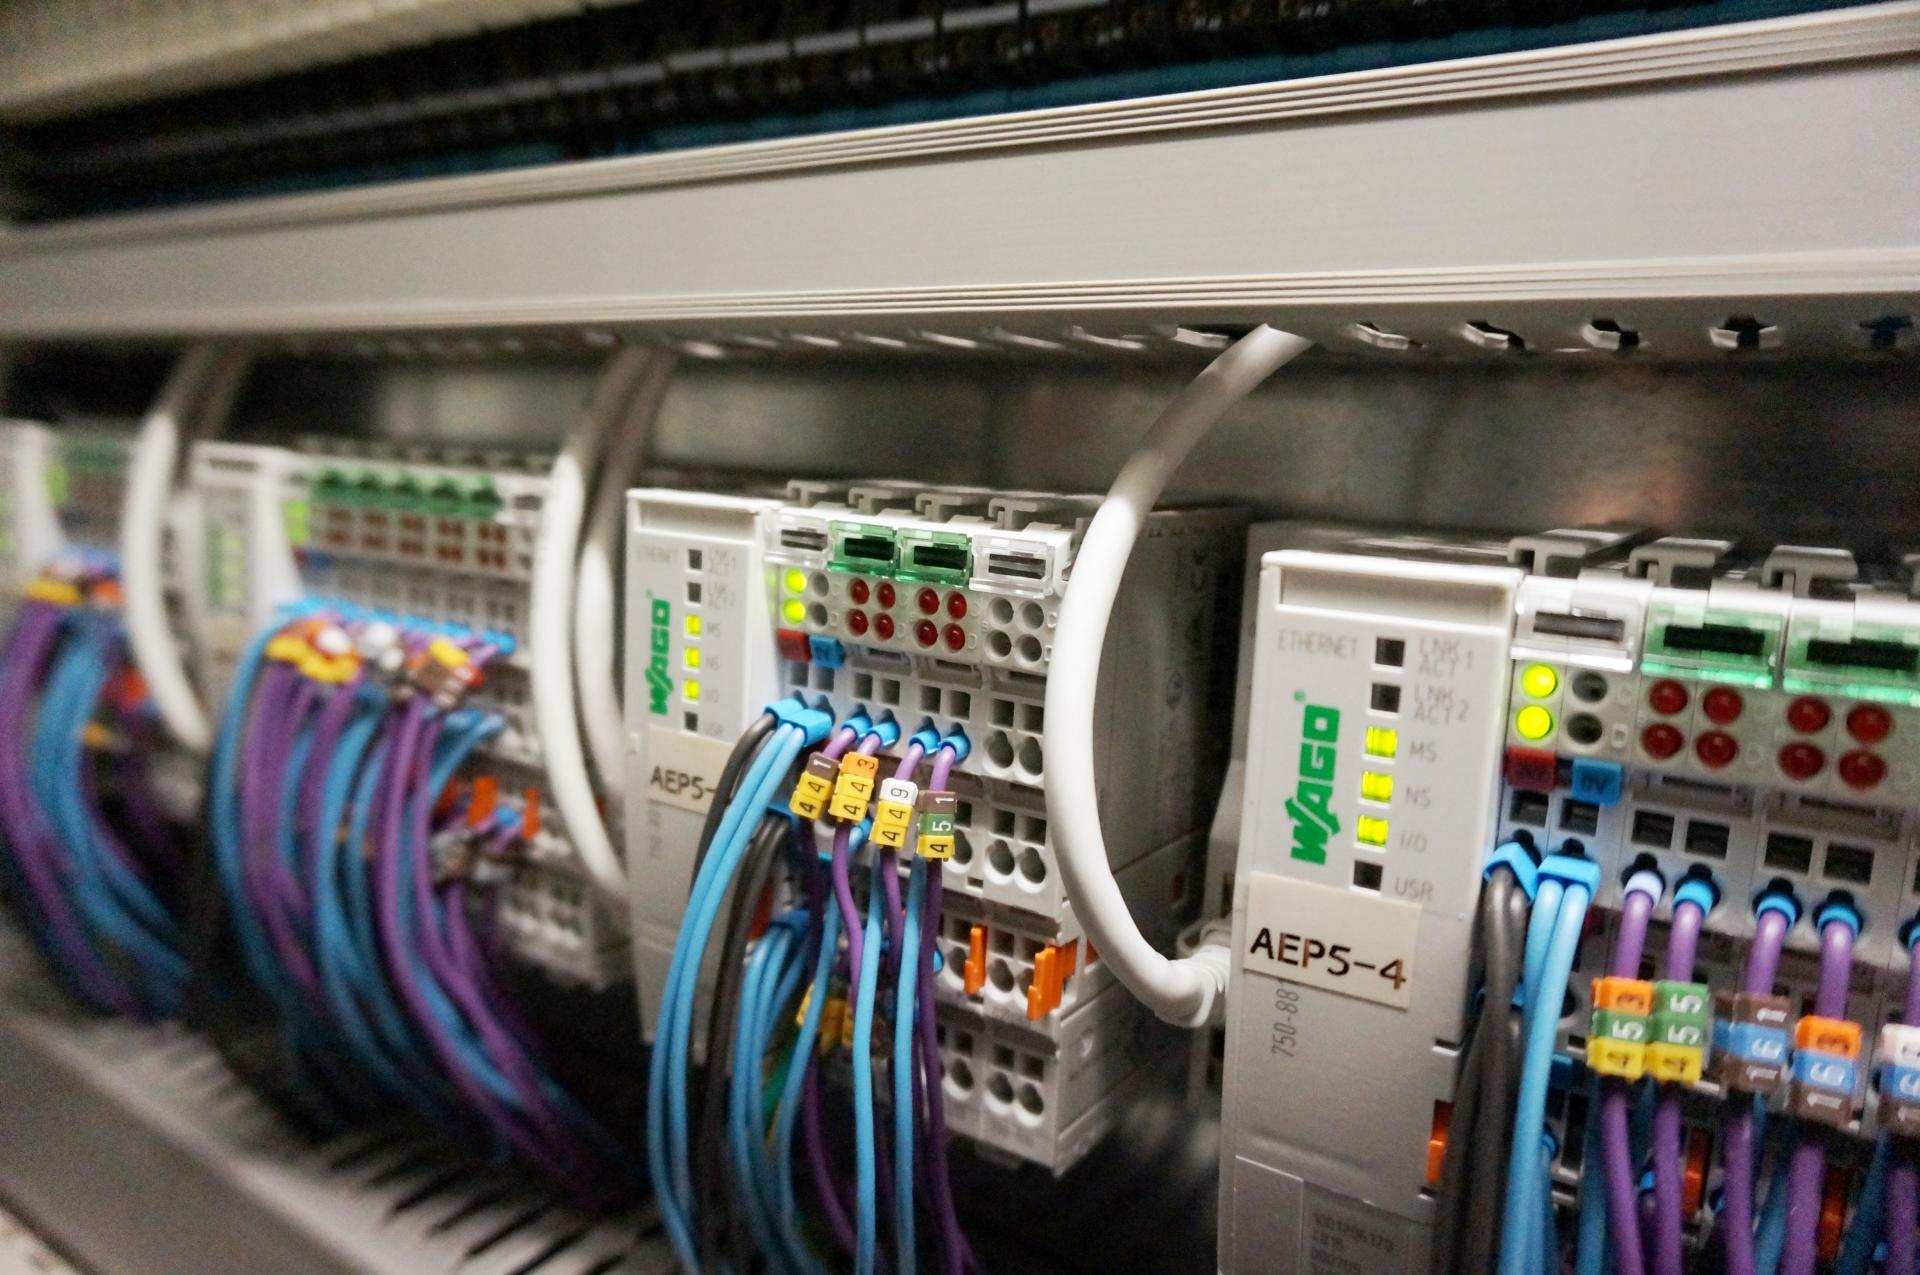
\includegraphics[width=0.7\textwidth]{data/plc.jpg}
\caption{Průmyslové \gls{plc} moduly. Převzato z~\texttt{wikimedia.org}.}
\label{fig:mtbusb-prototype}
\end{figure}

V~této práci se zaměříme na podmnožinu \gls{plc} modulů – totiž na takové,
jejichž hlavním úkolem je správně zpracovávat vstupní signály a~ovládat výstupní
periferie. Řízení logiky průmyslového procesu přenecháme počítači, s~kterým
\gls{plc} moduly komunikují.\footnote{V~praxi může \gls{plc} modul řídit logiku
procesu přímo, my však tuto situaci zkoumat nebudeme.}

Cílem této práce je navrhnout a implementovat novou verzi komunikační sběrnice
\gls{plc} obvodů \textit{\gls{mtbbus}} (\textit{Model Train
Bus}\footnote{Expanze zkratky do jejího plného významu nedává smysl, i~tak
budeme používat označení MTBbus, protože tak je zkratka zaužívaná.}).

\gls{mtbbus} je sběrnice, která se využívá pro řízení modelových kolejišť.
Je součástí systému \gls{mtb}. Skrze sběrnici lze číst signály z~kolejiště
(například polohy výhybek, obsazenost kolejových obvodů) a~povelovat prvky
v~kolejišti (návěstidla, přestavníky výhybek, přejezdy apod.). Obdobným
způsobem funguje zapezpečovací zařízení na skutečné železnici.

V~této práci autor nejprve popíše současné nasazení systému \gls{mtb}. Budou
formulovány důvody vedoucí k~nutnosti aktualizace sběrnice. Autor popíše, proč
jsou dostupná komerční řešení nevhodná a~navrhne vlastní nové (1) protokoly,
(2) hardwarové moduly a~(3) počítačové programy, které jím formulovaný problém
řeší.


\chapter{Současné nasazení sběrnice MTBbus} \label{chap:nasazeni}
Sběrnice \gls{mtbbus} vznikla okolo roku 2000, kdy se hledal vhodný systém pro
programovatelné počítačové řízení modelové železnice, spoluprací nadšenců
z~\textit{Klubu modelářů železnic Brno I} (dále jen \gls{kmz}) a \textit{Klubu
železničních modelářů Praha 3} \footnote{Je překvapivé, že
skupina nadšenců tehdy dokázala vytvořit systém, který by se mohl poměřovat se
současnými komerčními systémy řízení modelových kolejišť, viz dále.} \cite{mtb:web}.

\textit{Digital Command Control} (\gls{dcc}), dnes pravděpodobně
nejrozšířenější\footnotemark\\mezinárodně standardizovaný systém pro digitální
řízení modelové železnice \cite{dcc_intro:web} tehdy ještě nebyl v~České Republice
rozšířený. Navíc přirozeně vyvstal požadavek na minimalizaci nákladů
a maximalizaci nezávislosti na komerčních produktech jediného výrobce. Vznikl
tedy systém \gls{mtb}, který se pro řízení modelových kolejišť v \gls{kmz}
používá doteď \cite{kmz_rizeni:web}. Podotkněme, že systém \gls{mtb} se
do~dalších klubů po České Republice nerozšířil – nejspíš proto, že není
podporovaný komerčními softwary pro řízení modelové železnice a~že jej jeho
původní autor v~roce~2008 přestal podporovat.

\footnotetext{Autor této práce by rád odstranil slovo
\textit{pravděpodobně} a uvedl řádnou citaci. Bohužel neexistují studie, které
by bylo možné mohli citovat. Rozšířenost \gls{dcc} se zakládá na autorových
zkušenostech.}

\section{Popis sběrnice \gls{mtbbus}} \label{sec:mtbbus}

Každé kolejiště má svou vlastní sběrnici \gls{mtbbus}, ke které je připojený
právě jeden \textit{\gls{mtbusb} modul} a až \textit{255 \gls{mtb} modulů}.
\gls{mtbusb} modul řídí provoz sběrnice \gls{mtbbus} a~je připojen k~počítači.
\gls{mtb} moduly jsou pevně instalovány v~rámech kolejiště a~komunikují po
sběrnici \gls{mtbbus} s~\gls{mtbusb} modulem. Říkáme, že sběrnice je tzv.
\textit{single master, multiple slaves}. \gls{mtbusb} modul lze označit jako
\textit{master modul}, \gls{mtb} moduly jsou tzv. \textit{slave moduly}.
Celou situaci přehledně ilustruje obrázek \ref{fig:mtbbus-topology}.

Každý \gls{mtb} modul má:

\begin{compactenum}
\item 8bitovou adresu, která se konfiguruje \textit{jumpery} přímo na modulu,
\item konfiguraci (typ vstupů/výstupů, rychlost sběrnice, ...),
\item vstupy (stav vstupů),
\item výstupy (stav výstupů).
\end{compactenum}


\begin{figure}[ht]
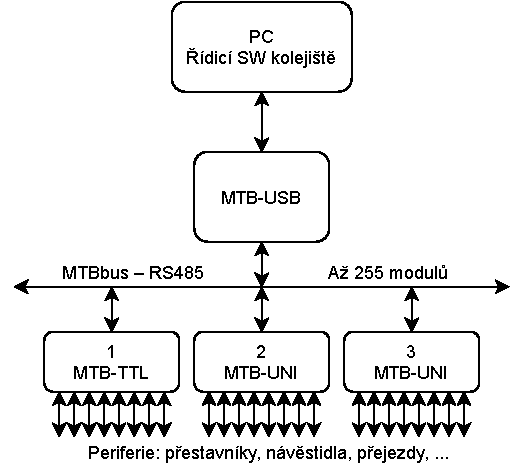
\includegraphics[width=0.7\textwidth]{data/mtb-topology.pdf}
\caption{Topologie systému \gls{mtb}.}
\label{fig:mtbbus-topology}
\end{figure}

\begin{table}[h]
	\begin{tabularx}{\textwidth}{XX}
		\toprule
		Typ přenosu & RS485, formát dat UART \\
		Komunikační rychlost & 38400~Bd, 57600~Bd, 115200~Bd \\
		Maximální počet modulů & 255 \\
		Počet datových bitů & 9 \\
		Stop bit & 1 \\
		Parita & žádná \\
		Maximální délka vedení & 100 m \\
		\bottomrule
	\end{tabularx}
	\caption{Základní parametry sběrnice \gls{mtbbus} \cite{mtbbus-specs}}
	\label{tab:mtbbus-params}
\end{table}

Současná sběrnice \gls{mtbbus} je založena na elektrickém standardu
\textit{RS485} \cite{mtbbus-specs}. Sběrnice RS485 je dvouvodičová (\textit{R+,
R-, GND}) vícebodová sériová poloduplexní komunikační průmyslová sběrnice
vyvinutá s~důrazem na odolnost vůči externímu rušení. Je vhodná pro přenos dat
na větší vzdálenosti, řádově až stovky metrů \cite{rs485-specs}. Pro dosažení
nejlepších elektrických vlastností by sběrnice měla být lineární. Sběrnice je
na obou koncích termínována rezistorem \textit{200 R} a~pull-up a~pull-down
rezistory pro držení definované úrovně signálu.

RS485 je velice snadno implementovatelná do prakticky všech mikrokontrolérů –
pro přístup ke sběrnici je třeba rozhraní UART, jeden pin pro řízení směru
komunikace a driver k~RS485.

\gls{mtb} moduly mohou být různého typu:

\begin{itemize}
\item \textbf{\gls{mtbuni}}

	\gls{mtbuni} (\textit{univerzální}) je nejpoužívanější typ modulu. Obsahuje
	16~digitálních vstupů a~16~digitálních výstupů. Na výstupech 0–7 umožňuje
	kódovat návěst protokolem S-COM\footnote{S-COM je jednoduchý jednosměrný
	komunikační protokol, který umožňuje přenášet návěsti návěstidel
	\cite{scom-specs}.}, což umožňuje připojení až 8 návěstidel k~jednomu
	\gls{mtbuni}. Modul dále umožňuje připojení IR čidel na
	vstupy\footnote{IR čidla jsou bodová čidla detekující průjezd vlaku, viz
	\ref{sec:ir}.}. Výstupy modulu jsou v~režimu otevřeného kolektoru
	s~maximální zátěží až 0.5~A~/~8~výstupů.

\item \textbf{MTB-TTL}

	\begin{figure}[ht]
	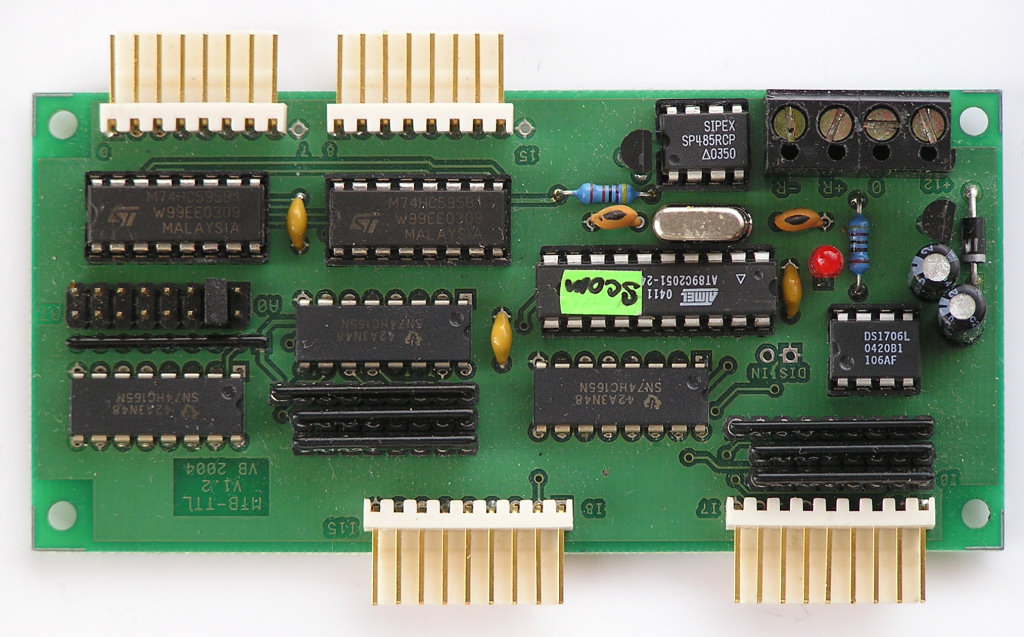
\includegraphics[width=0.7\textwidth]{data/mtbttl_foto.jpg}
	\caption{Ukázka modulu MTB-TTL \cite{mtb:web}.}
	\label{fig:mtbttl}
	\end{figure}

	MTB-TTL je zjednodušením modulu \gls{mtbuni}. Oproti \gls{mtbuni}
	nemá podporu IR čidel a~výstupy má v~režimu \gls{ttl}. Od tohoto typu
	modulu se v~současnosti ustupuje, neboť \gls{ttl} výstupy nejsou vhodné pro
	spínání vyšších napětí\footnote{např. pokud periferie na výstupu obashuje
	pull-up do +12~V} a~proto, že v~případě neaktivního výstupu (neaktivní =
	+5~V; inverzní logika) aktivně napájí výstupní port, což způsobuje nechtěné
	chování, například pokud je ne výstupním portu záměrně vypnutá periferie.
	V~krajním případě může dojít až k~přetížení TTL výstupu a jeho zničení. Na
	všechny nasazené moduly typu MTB-TTL byly postupně instalovány dodatečné
	obvody s~otevřenými kolektory na výstupy.

\item \textbf{MTB-REG}

	MTB-REG je modul umožňující generovat analogový výkonový výstup. Modul se
	připojí ke kolejím a řídí rychlost a~směr lokomotivy v~řízeném úseku kolejí.

	Tento způsob řízení jízdy (tzv. \textit{analogový}) je dnes již překonaný.
	V~současnosti se pro řízení jízdy lokomotiv na kolejišti používá tzv. systém
	\textit{Digital Command Control} (viz \ref{sec:dcc}), kde každá lokomotiva
	a mnohdy i~vagón v~sobě má mikroprocesor a~celý systém je řízen
	digitálně \cite{dcc_intro:web}.

	Modul MTB-REG je tedy již překonaným modulem a autor jej uvádí spíš pro
	úplnost popisu systému \gls{mtb}.

\item \textbf{MTB-POT}

	Modul MTB-POT obsahuje 4 analogové vstupy a 4 digitální vstupy. Jeho
	původním účelem bylo, aby se připojil k~potenciometru v~pultu obsluhy
	kolejiště, kterým obsluha reguluje jízdu vlaku. Po sběrnici přepošle data
	modulu MTB-REG a~tím dojde ke kýžené jízdě vlaku. Tento způsob řízení jízdy
	na kolejištích se již nepoužívá, proto i~modul MTB-POT na moderních
	kolejištích pozbývá svého smyslu.

\end{itemize}

Po sběrnici se komunikuje pevně definovaným protokolem.  Protokol definuje
příkazy pro moduly, odpovědi modulů, časování apod \cite{mtbbus-specs}.

Práce se sběrnicí z~pohledu aplikace v~počítači probíhá následovně:

\begin{compactenum}
\item Aplikace se připojí se k~MTB-USB modulu.
\item Aplikace provede sken aktivních modulů sběrnice.
\item Aplikace nahraje do všech aktivních modulů konfiguraci.
\item Aplikace přečte stav vstupů.
\item Aplikace zahájí provoz sběrnice – od této chvíle všechny moduly nahlašují
	změny stavů vstupů.
\item Aplikace čte vstupy, nastavuje výstupy a řídí provoz.
\item Aplikace ukončí provoz sběrnice a vynuluje stav výstupů \gls{mtb} modulů.
\item Aplikace uzavře spojení s~MTB-USB.
\end{compactenum}


\section{IR čidla} \label{sec:ir}

Nyní popíšeme princip fungování IR čidel v~kolejišti, protože bude v~dalších
kapitolách stěžejní.

IR čidlo je bodový detektor průjezdu vlaku. Do kolejí se vedle sebe umístí
opticky oddělená vysílací dioda a~fototranzistor, oba namířené vzhůru. Při
průjezdu vlaku dojde k~odrazu signálu od spodku vozu nebo lokomotivy, čímž je
detekován průjezd vlaku. Výhodou je nenápadná instalace mezi pražce, která
neruší celkový dojem modelu.

Pro spolehlivou detekci odrazu od matných černých povrchů podvozků je třeba
budit vysílací diodu vysokým proudem (až 200~mA), což vyžaduje použití
diody v~impulsním režimu. Současná \gls{mtbuni} deska podporuje IR čidla na
všech svých 16 vstupech, diody jsou buzeny tranzistory ve skupinách po
4~diodách.

\begin{figure}[ht]
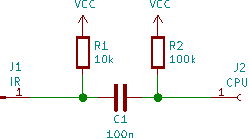
\includegraphics[width=0.5\textwidth]{data/cap-bind/capacitive-bind-example.pdf}
\caption{Zapojení vstupu kapacitní vazbou.}
\label{fig:cap-bind}
\end{figure}

Aby bylo zajištěno spolehlivé vyhodnocení odraženého signálu, je vstup
z~fototranzistoru zapojen na digitální vstup posuvného registru přes kapacitní
vazbu.

Vstupy \gls{mtbuni} desky se konfigurují osazením rezistorových lišt (běžný
vstup) nebo kondenzátorů (vstup z IR čidla). Kromě toho musí o~režimu pinu
vědět i~procesor, aby adekvátním způsobem zpracovával vstupní signál
\cite{mtbuni22-specs}.


\section{Systém \gls{mtb} v~kontextu řízení celého kolejiště} \label{sec:mtb_context}

V~\gls{kmz} je aktuálně systém \gls{mtb} nasazen na dvou kolejištích, další
nasazení je na modulovém kolejišti Mendelovy univerzity v~Brně, s~kterou klub
spolupracuje. Na těchto kolejištích je aktuálně nasazeno 99 \gls{mtb} desek.

Pro kontext uveďme, jak systém \gls{mtb} zapadá do celkové koncepce řízení
kolejiště. Viz schéma \ref{fig:control-topology}.

\begin{figure}[ht]
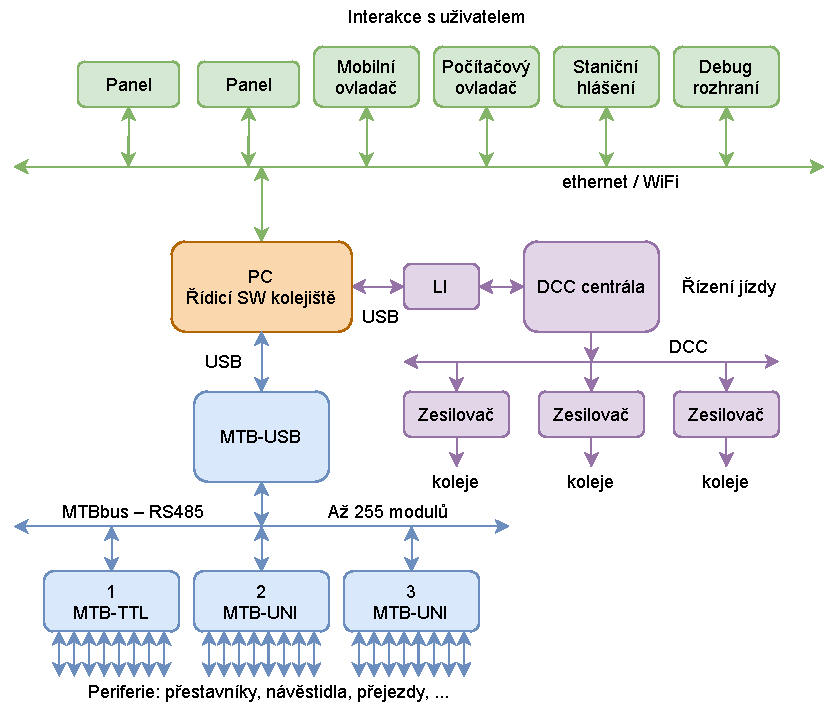
\includegraphics[width=\textwidth]{data/railroad-topology.pdf}
\caption{Schéma komponent řízení kolejiště v~\gls{kmz}.}
\label{fig:control-topology}
\end{figure}

Na první pohled je vidět, že kolejiště je řízeno dvěma různými systémy (modrá
a~fialová část diagramu).  Vyvstává otázka, proč je neintegrovat do systému
jednoho. Integrovaná řešení nabízejí majoritní výrobci hardwaru pro digitální
řízení modelové železnice.  Řízení jízdy i~trakce jedním systémem (\gls{dcc})
je rozšířeným přístupem jak v~Česku tak v~zahraničí. Všechna tato řešení jsou
však o~kompromisech, jak se dozvíme v~\ref{sec:dcc}. U~tvorby a~nasazení
systému \gls{mtb} stály osoby, které pracují na zabezpečení skutečné železnice.
Systém \gls{mtb} je tak oproti komerčně dostupným řešením řízení modelových
kolejišť navrhován s~důrazem na spolehlivost a~především bezpečnost.

Uveďme dva příklady za všechny: komerčně využívaná sběrnice RS pro snímání
stavu kolejiště nedokáže rozpoznat, že nějaký z~RS modulů (analogie \gls{mtb}
modulů) přestal fungovat \cite{rs:web}. Dále výstupní moduly nijak nepotvrzují,
že opravdu provedly akci, kterou počítač požaduje \cite{dcc_specs:web}. Tyto
příklady ilustrují, že komerčně dostupná řešení jsou podle autorova názoru blíže
hračce, než bezpečnému a~spolehlivému systému pro řízení modelů.

Poslední část schématu \ref{fig:control-topology} je část zelená, která
reprezentuje interakci s~uživatelem. \textit{Řídicí SW kolejiště} běží na
samostatném serveru, ke kterému se připojují všichni uživatelé systému –
dispečeři ze svých stanic, strojvedoucí ze svých ovladačů ale také třeba
technikové se svými diagnostickými nástroji nebo externí programy využívající
API serveru. Server kontroluje identitu uživatelů a umožňuje jim řídit ty
systémy, ke kterým mají uživatelé práva.

\section{Proč současný systém \gls{mtb} nedostačuje} \label{sec:mtb_fail}

Systém \gls{mtb} s~sebou nese řadu problémů.

\begin{enumerate}
\item \textbf{Licence, výrobní data}

U~současné implementace systému \gls{mtb} bohužel nebyly řádně vyřešeny licenční
podmínky mezi jeho autorem a~klubem. Souhrou událostí se \gls{kmz} dostal do
situace, kdy nemáme zdrojová data schémat a~layoutů desek plošných spojů ani
zdrojové kódy firmwarů.

Aktuální situace tak prakticky znemožňuje výrobu dalších \gls{mtb} desek,
o~záměru chtít systém \gls{mtb} nabízet mimo klub ani nemůže být řeč.

\item \textbf{Hardware}

Systém \gls{mtb} zaznamenal poslední aktualizaci hardwarových komponent v~roce
2007. V~současné době jsou některé použité součástky bohužel prakticky
nesehnatelné, což znemožňuje výstavbu dalších částí kolejiště. To je zcela
zásadní problém.

\item \textbf{Software}

Současné MTB moduly využívají procesory \textit{AT89C2051} (2~kB FLASH,
128~B SRAM). Tyto procesory svými parametry odpovídají době návrhu celého
systému. Firmware v~procesorech naráží na jejich hardwarové limity – do
procesoru se jednoduše nevejde další logika, což efektivně zabraňuje přidání
nových funkcí. Procesorům navíc chybí některé klíčové periferie, například
EEPROM paměť.

\end{enumerate}

Současný systém \gls{mtb} byl vyhodnocen jako celkově nedostatečný, je potřeba
ho buď aktualizovat nebo nahradit za systém jiný.

Na náhradu systému \gls{mtb} autor práce stanovil především následující
požadavky.

\begin{compactenum}
\item Systém musí být kompatibilní se současným řídicím softwarem kolejiště.
\item Systém musí být kompatibilní se současným hardwarem kolejiště.
\item Systém musí být udržitelný minimálně 20~let.
\item Finanční náklady a~čas vložený do povýšení současného systému na nový
	systém by měly být minimalizovány.
\item Systém musí být schopen potvrzovat akce řídicího počítače a~evidovat správnou
	funkčnost modulů.
\item Systém by měl být rozšiřitelný co se týče podporované funkcionality –
	nové požadavky na funkcionalitu by mělo být možné implementovat.
\end{compactenum}

K~naplnění těchto požadavků lze přistoupit dvěma různými způsoby: zakoupením
komerčního produktu nebo vytvořením produktu vlastního. Prozkoumejme nejprve,
jestli existují komerční řešení, která naplňují definované požadavky.


\chapter{Závěr} \label{chap:zaver}
Tato diplomová práce demonstrovala, že pro vytvoření plnohodnotného \gls{plc}
systému je třeba zvládnout širokou škálu dílčích kroků. Od návrhu komunikačních
protokolů, přes návrh hardwaru, programování firmwaru, až po programování
počítačových aplikací a~knihoven. Autorovi se povedlo všechny tyto kroky
úspěšně provést. Podařilo se mu vytvořit

\begin{compactitem}
\item nový protokol \gls{mtbbus},
\item nový master modul sběrnice \gls{mtbbus} (\gls{mtbusb} v4),
\item nový univerzální \textit{slave} modul sběrnice \gls{mtbbus} (\gls{mtbuni} v4),
\item nástavný modul do starších modulů \gls{mtbuni} (MTB-2-AVR),
\item počítačovou aplikaci pro přístup k~systému \gls{mtb} (MTB Daemon),
\item knihovnu pro integraci nového \gls{mtb} do současného řídicího systému
	kolejiště (hJOP MTB Network RCS Library)
\end{compactitem}

Komponenty vytvořené v~rámci této práce a~jejich interakce jsou přehledně
zobrazeny v~\ref{fig:new-topology}.

\begin{figure}[ht]
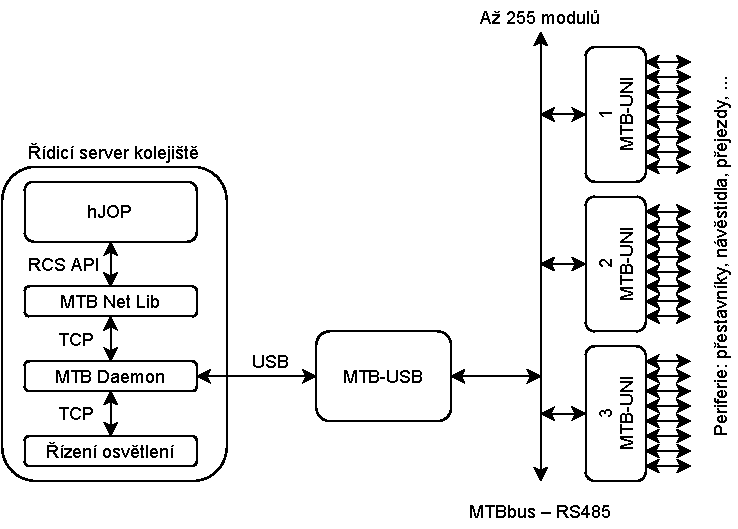
\includegraphics[width=0.8\textwidth]{data/new-topology.pdf}
\caption{Komponenty vytvořené v~rámci diplomové práce (mimo \textit{hJOP}
a~\textit{Řízení osvětlení}).}
\label{fig:new-topology}
\end{figure}

V~rámci práce byly formulovány požadavky (\ref{sub:mtbbus-req-summary}), které
má nový systém \gls{mtb} splnit. Všechny tyto požadavky byly naplněny.
Podařilo se vytvořit systém, který za poměrně malé finanční a časové náklady
značně povyšuje současný systém \gls{mtb}. Především však vznikl otevřený
a rozšiřitelný systém s~výhledem udržitelnosti po desítky let. Nový systém
\gls{mtb} umožní stavbu dalších kolejišť, udržování a rozšiřování kolejišť
současných. Nový systém \gls{mtb} si může vyrobit každý, kdo bude chtít bezpečně
řídit své modelové kolejiště.

Pro \gls{kmz} znamená \gls{mtb} v4 možnost nasadit více řídicích systémů
kolejiště, a~konečně tak zprovoznit řízení osvětlení, řízení tramvajové
a~autobusové dopravy. \gls{mtb} v4 umožní nasazení pultů obsluhy,
vytvoření nových chytrých zesilovačů \gls{dcc} signálu. Umožní výstavbu nového
depa kolejových vozidel, kde se budou používat speciální \gls{mtb} moduly.
Pro \gls{kmz} je \gls{mtb} v4 velkým krokem vpřed.

\gls{mtb} v4 bylo nasazeno na testovacím kolejišti o~20 modulech, kde úspešně
funguje.

\section{Možná rozšíření} \label{sec:future}

Při návrhu tak velkého systému, jako je \gls{mtb}, se přirozeně ukázaly mnohé
cesty, které by bylo možné v~budoucnu prozkoumat.

Systém \gls{mtb} by v~budoucnu mohl podporovat vyšší rychlosti komunikace nebo
automatickou detekci rychlosti sběrnice. \gls{mtb} by mohlo být rozšířeno
o~jednotky, které provádějí retranslaci dat sběrnice bezdrátově (pro vzdálené
připojení modulů).

Jednou z~otázek týkajících se budoucího rozšíření je, jak umožnit, aby systém
\gls{mtb} mohl interagovat s~komerčními softwary pro řízení modelových
kolejišť.
Dalším možným rozšířením je tak implementovat do majoritních komerčních
softwarů pro řízení modelových kolejišť podporu pro \gls{mtb}. Některé softwary
jsou však uzavřené. Pro takové softwary by bylo možné napsat alternativní
firmware do \gls{mtbusb}, který by zajistil, že \gls{mtbusb} modul se pro
počítač bude tvářit jako některý z~komerčních systémů pro řízení kolejišť.

Dalším přirozeným způsobem rozšíření, který má autor této práce v~plánu
v~nejbližším roce uskutečnit, je přidání dalších typů modulů. V~budoucnu
vzniknou \gls{mtb} moduly pro chytré zesilovače \gls{dcc} signálu,
\textit{RailCom} detektory a jiné. Systém \gls{mtb} je na tato rozšíření
připraven.


\printbibliography[heading=bibintoc]

\appendix
\chapter{Přílohy} \label{chap:appendix}
\vspace{-2em}

\begin{figure}[H]
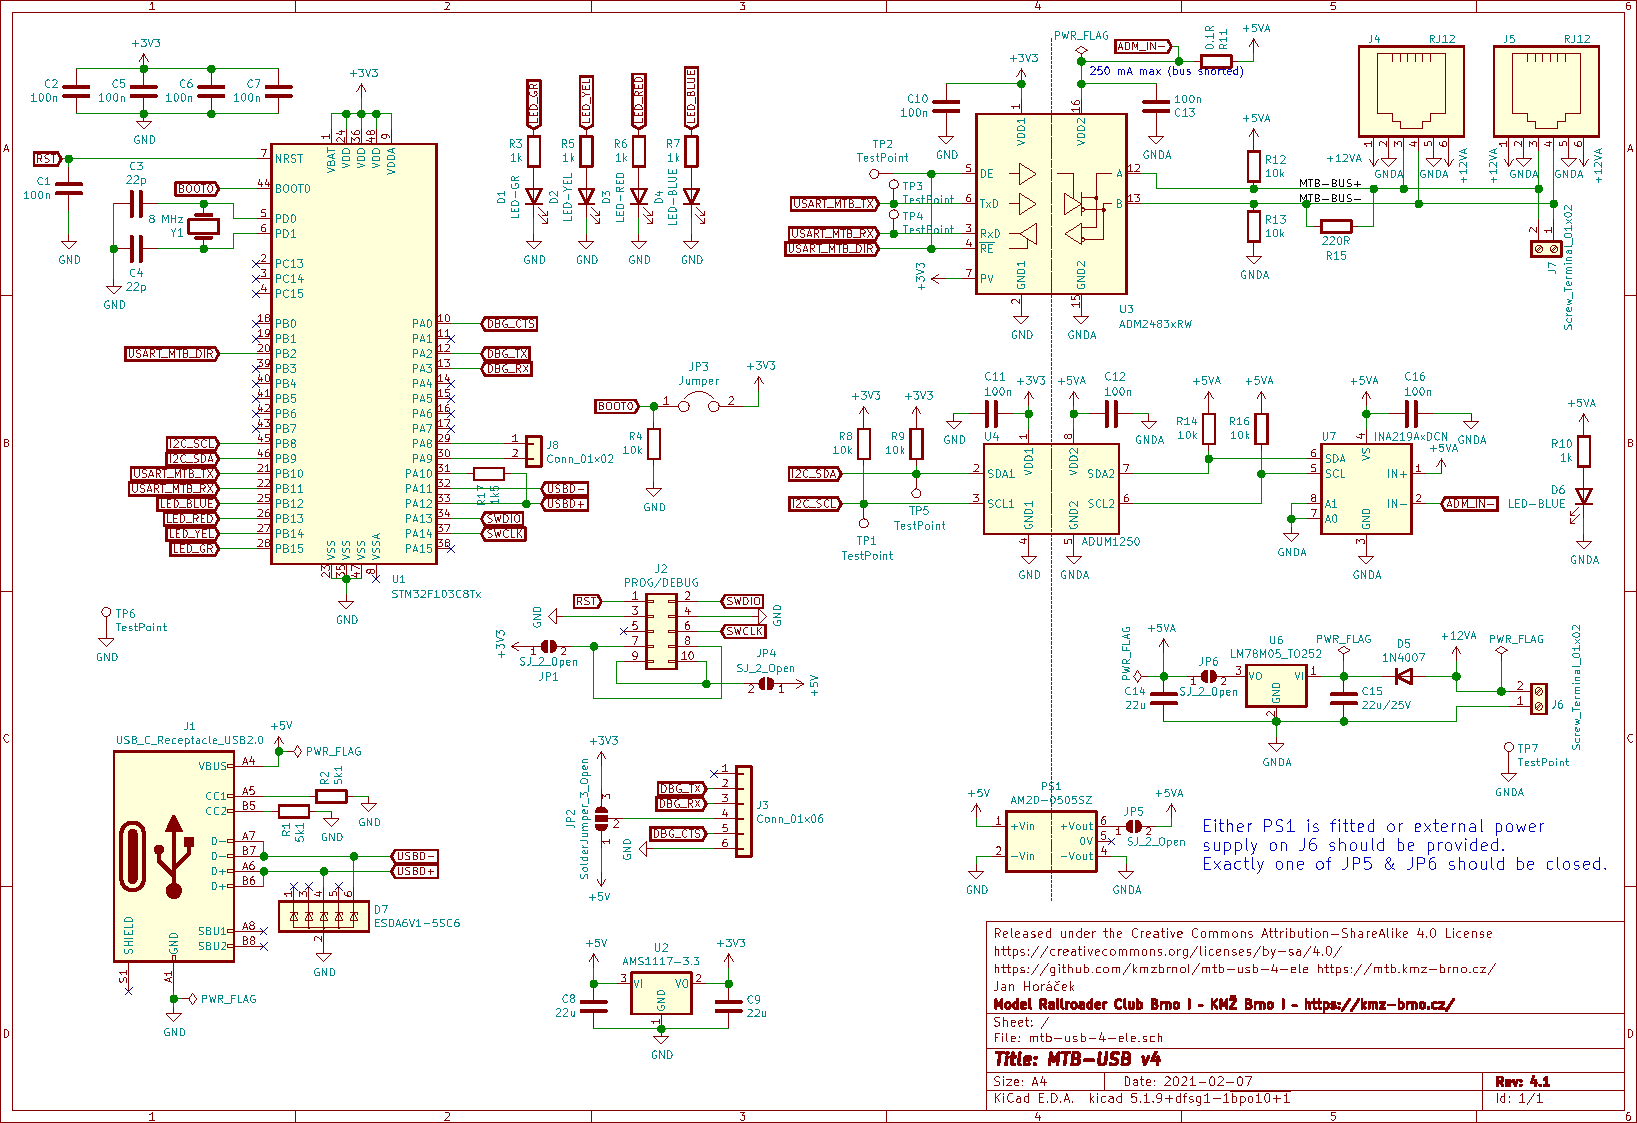
\includegraphics[angle=90,width=\textwidth]{data/mtb-usb-4-ele.pdf}
\caption{Schéma \gls{mtbusb} modulu.}
\label{fig:mtb-usb-sch}
\end{figure}

\begin{figure}[ht]
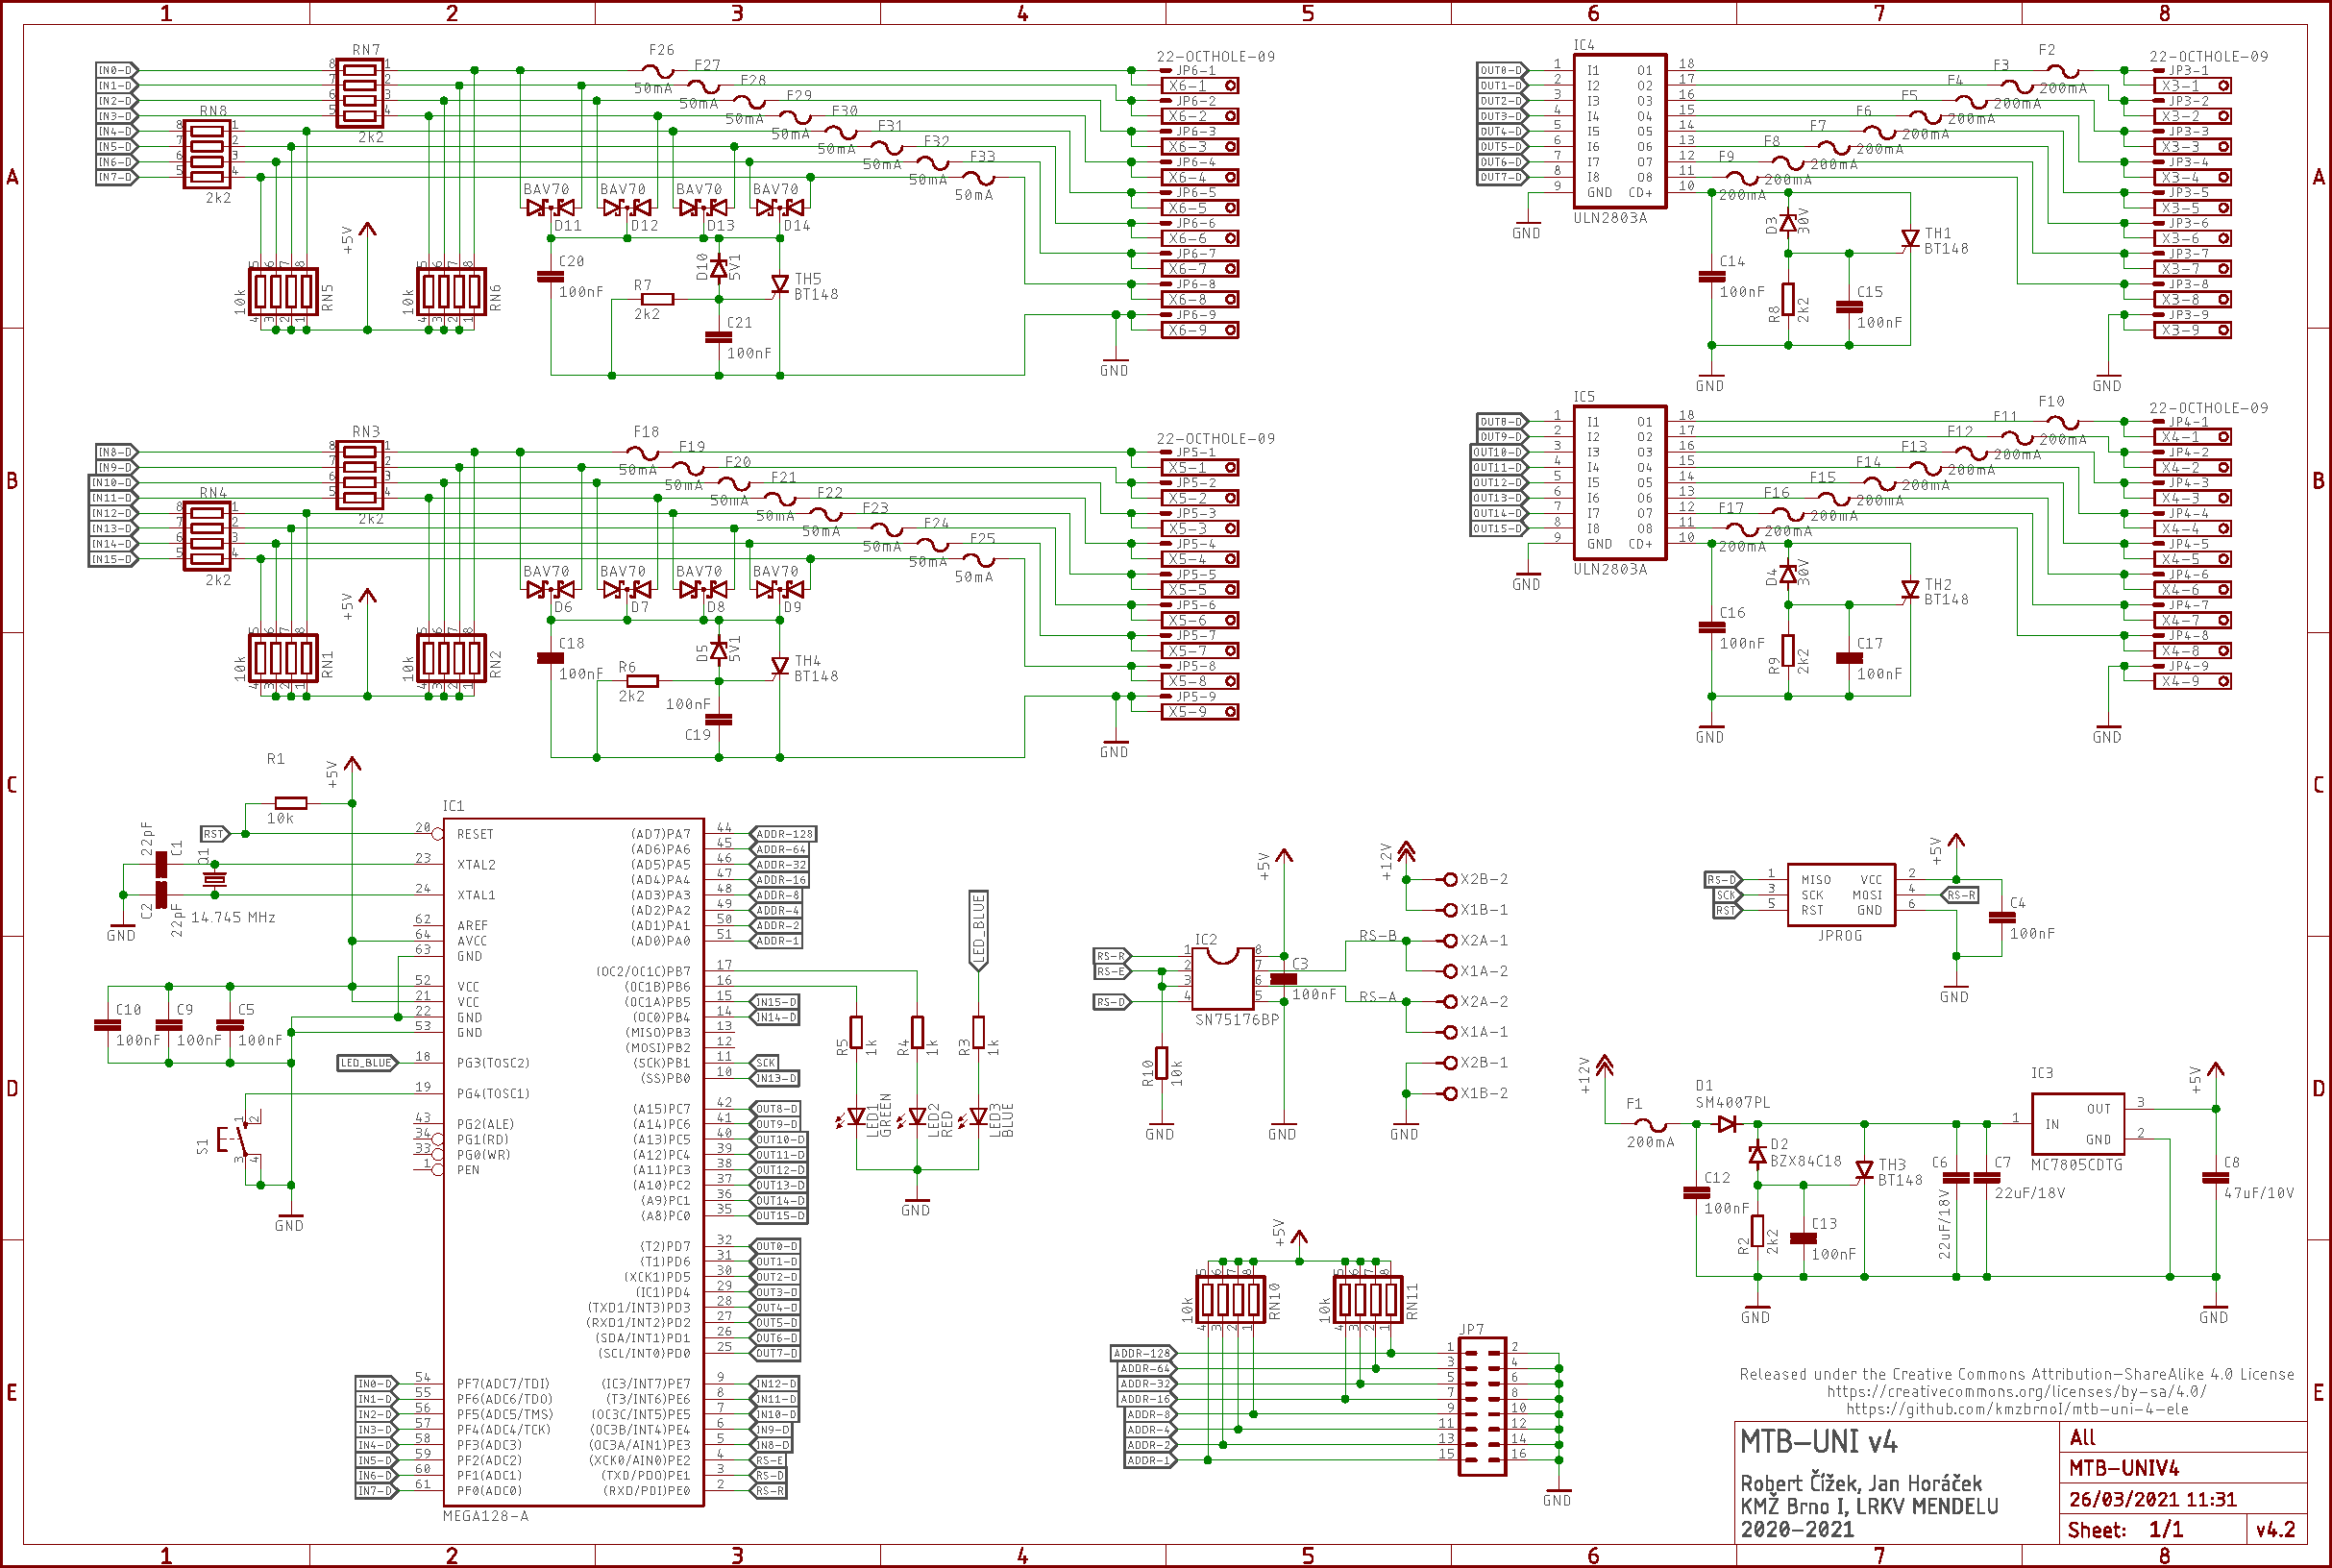
\includegraphics[angle=90,width=\textwidth]{data/mtb-uni-4-ele.pdf}
\caption{Schéma \gls{mtbuni} v4 modulu.}
\label{fig:mtb-uni-4-sch}
\end{figure}

\begin{figure}[ht]
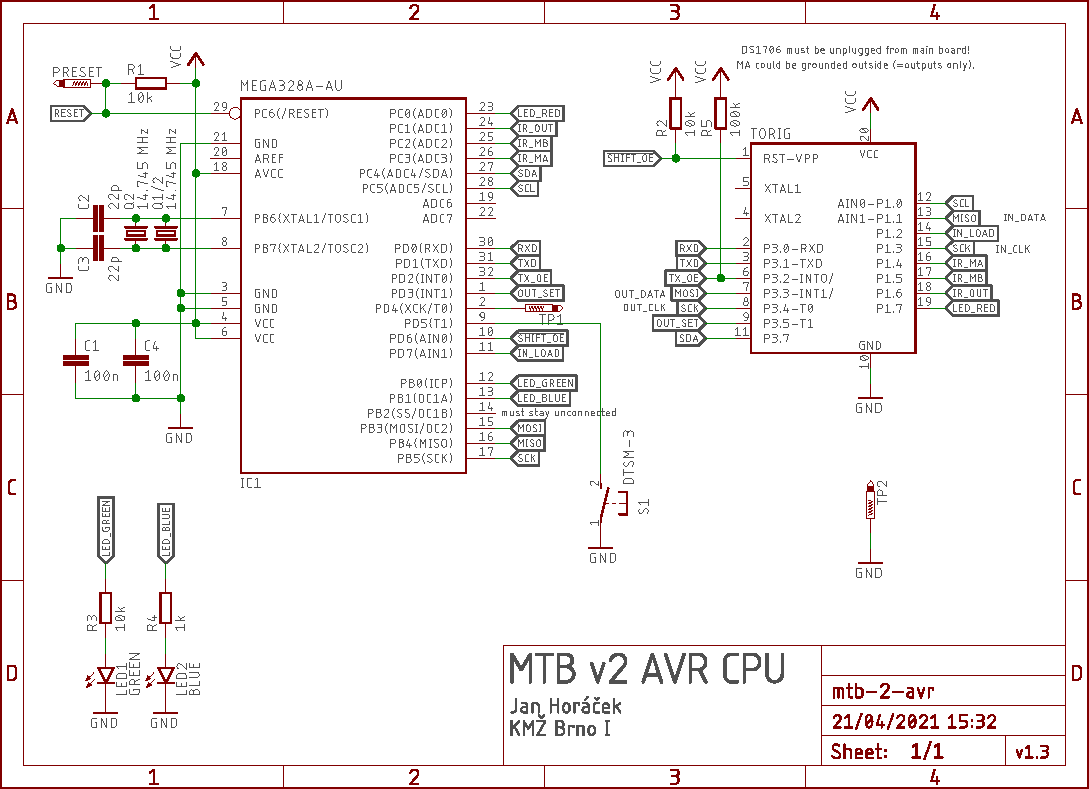
\includegraphics[angle=90,width=\textwidth]{data/mtb-2-avr-ele.pdf}
\caption{Schéma nástavné desky \textit{MTB-2-AVR}.}
\label{fig:mtb-uni-2-avr-sch}
\end{figure}

\begin{figure}[ht]
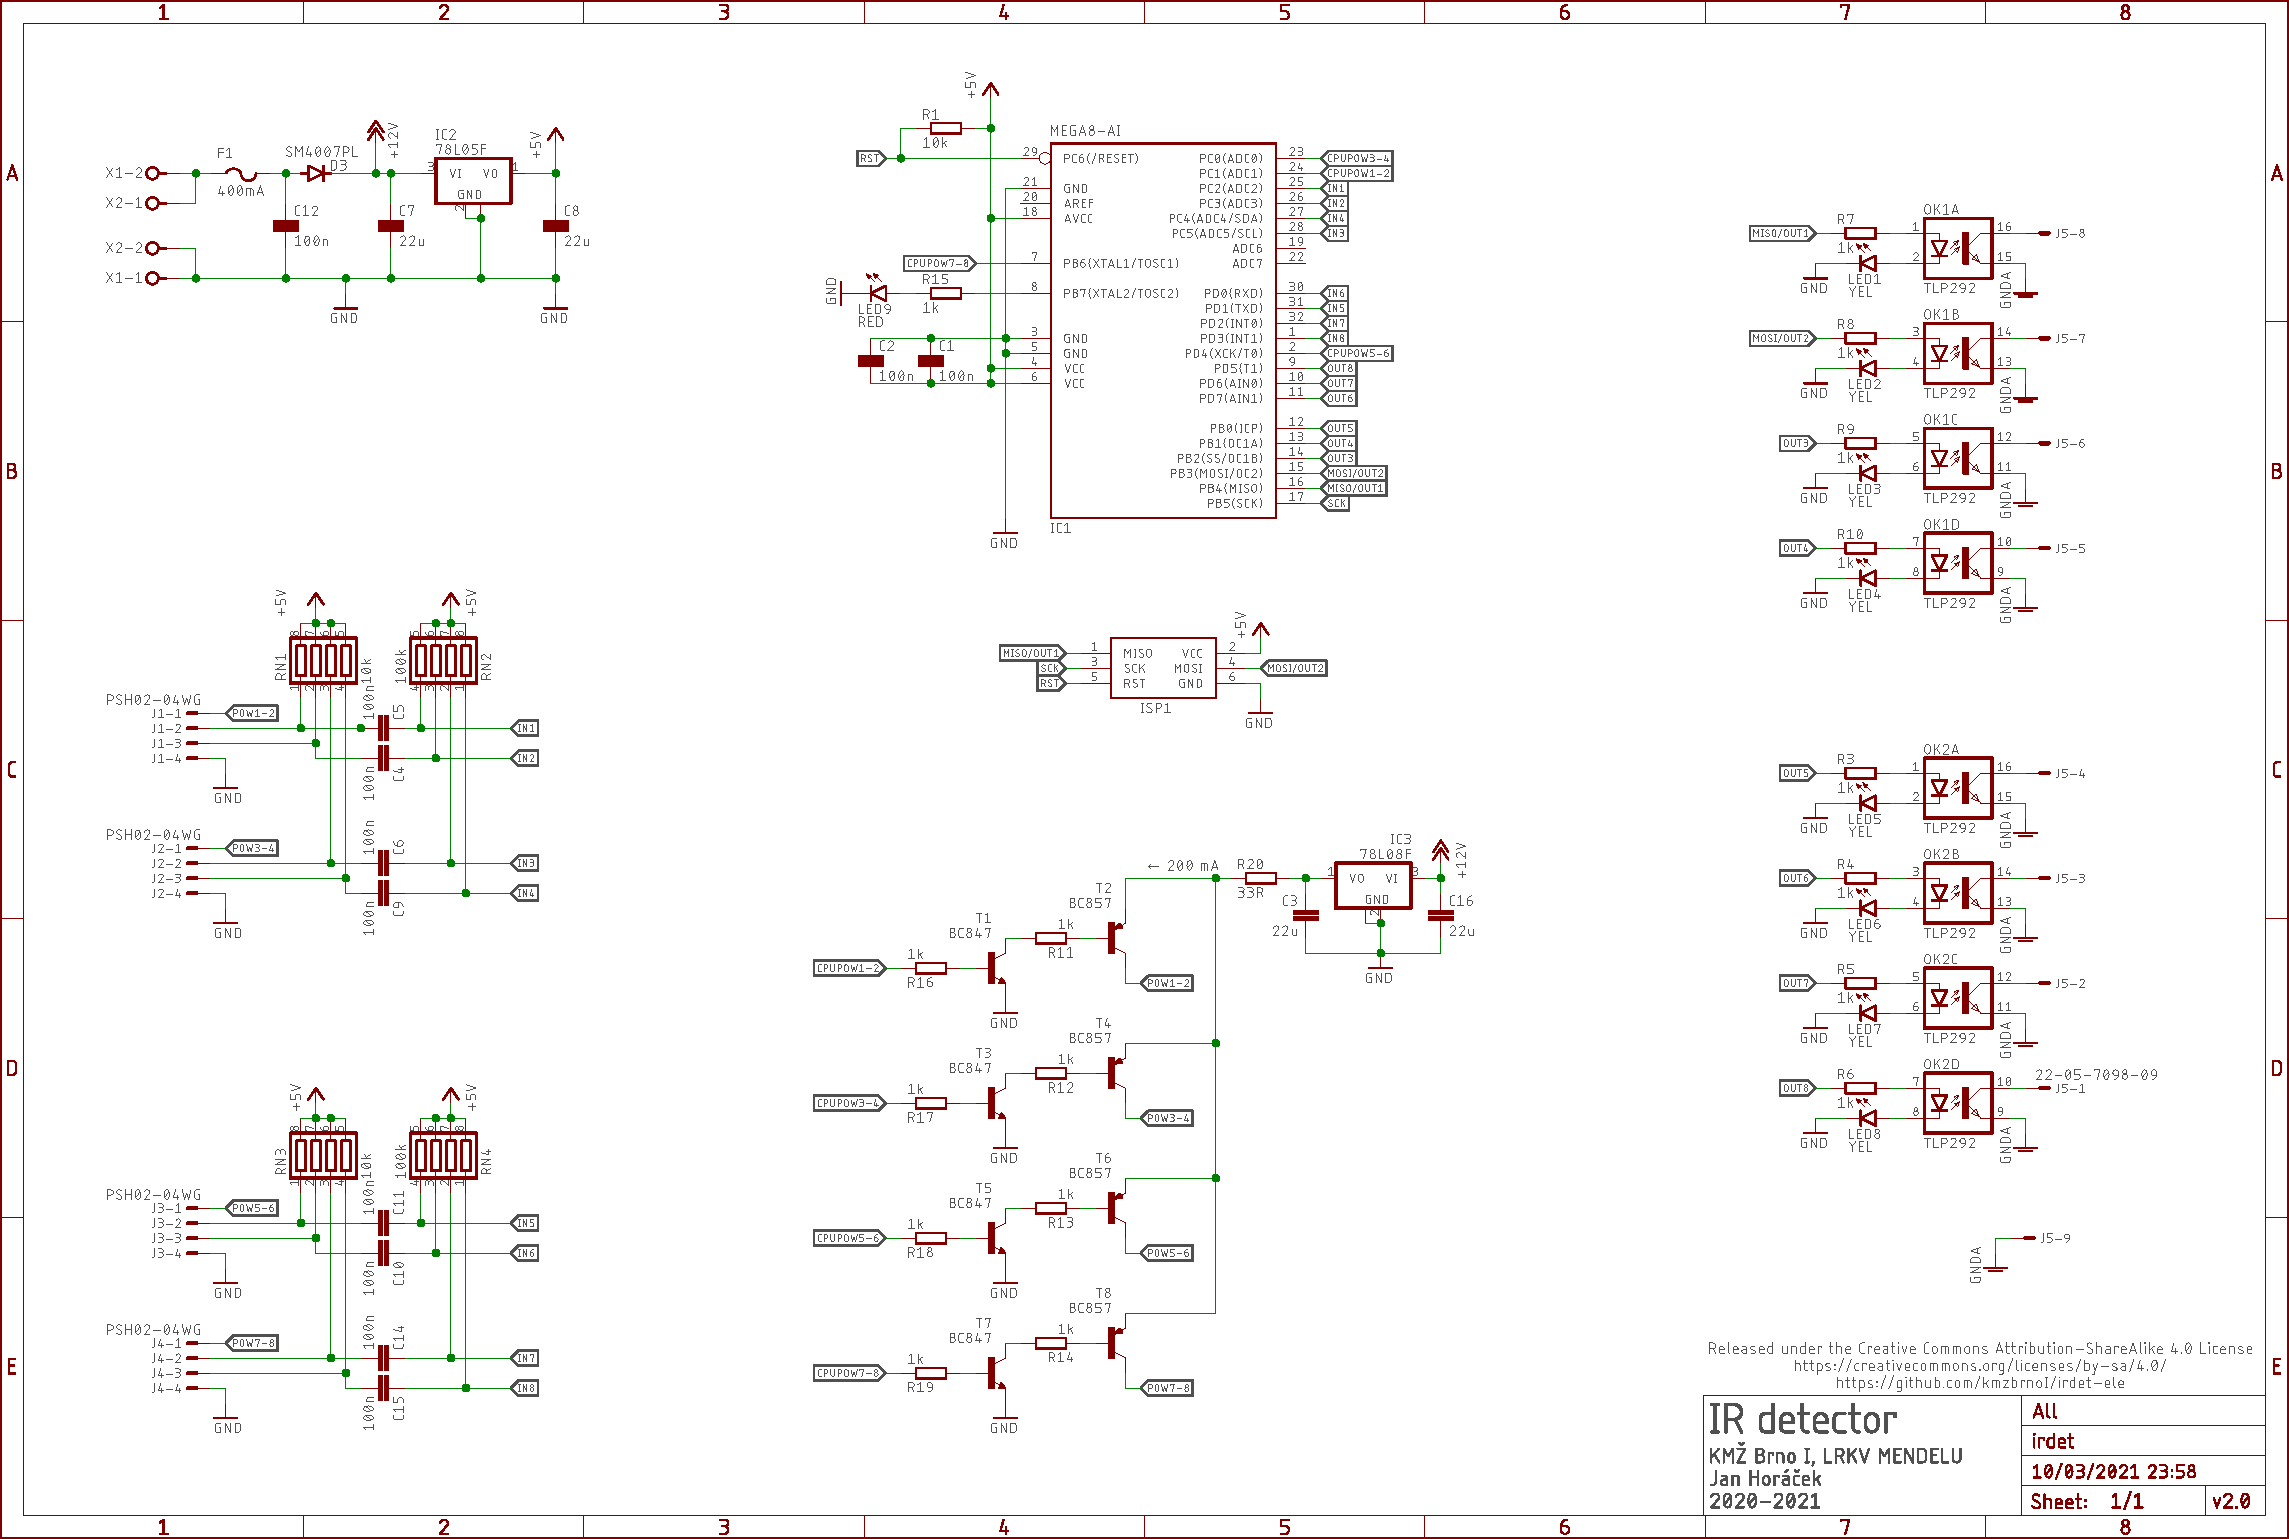
\includegraphics[angle=90,width=\textwidth]{data/irdet-ele.pdf}
\caption{Schéma desky \textit{IRdet}.}
\label{fig:irdet-sch}
\end{figure}


\end{document}
